\section{Experiment}
The experiment aims at using reinforcement learning algorithms for controling the solid-state lidar with a limited number of steerable rays. For purposes of the experiment it was neccessary to implement an environment, where an agent can learn and be evaluated \cite{rozsypalek2018}. The lidar-gym environment is written in Python 3 based on OpenAI gym interface \cite{openai2016}. It uses point clouds from the KITTI dataset drives\cite{geiger2013}. One episode of the learning in the environment corresponds to a drive in the KITTI dataset. The large point clouds from the drives are processed into 3D voxel maps by C++ package \cite{petricek2017}, which also provides a ray tracing engine for the environment. Every voxel map is a 3D array containing real numbers which correspond to the occupancy confidence $c$ of each voxel.
\begin{align}
\begin{split}
c &> 0 \quad \text{occupied voxel} \\
c &= 0 \quad \text{unknown occupancy} \\
c &< 0 \quad \text{empty voxel.}
\end{split}
\end{align}

\subsection{Environments}
Lidar-gym implements several environments (visualized in Figure \ref{fig:visualization}), which follow the same template with different sizes of the voxel maps.The observation space is a local cutout of the voxel map, which provides occupancies from sparse measurements of the sensor. The sensor is located in the quarter of x-axis and half of y-axis and z-axis of the local cutout. The action space is divided into two parts. The first part is the dense voxel map reconstructed from the observations (sparse measurements). The second part of the action space are directions of the measuring rays. Each ray has an own azimuth and elevation. The environment expects directions in the format of a 2D array of booleans, where true means a fired ray. The reward function of the environment is negative logistic loss $-L$ \eqref{eq:loglos}. Parameters of the environments are described in Table \ref{tab:envs}.

\begin{table}[H]
\centering
\begin{tabular}{|c||c|c|c|} 
\hline
Name of environment     & Large                        & Small                        & Toy                       \\ \hline
Voxel map size [voxels] & 320 $\times$ 320 $\times$ 32 & 160 $\times$ 160 $\times$ 16 & 80 $\times$ 80 $\times$ 8 \\ \hline
Lidar FOV [\textdegree]           & 120 $\times$ 90              & 120 $\times$ 90              & 120 $\times$ 90           \\ \hline
Densitiy of rays        & 160 $\times$ 120             & 120 $\times$ 90              & 40 $\times$ 30            \\ \hline
Lidar range [m]         & 42                           & 42                           & 42                        \\ \hline
Number of rays          & 200                          & 50                           & 15                        \\ \hline
Voxel size [m] & 0.2 & 0.4 & 0.8 \\ \hline
Episode training time [min]\footnotemark{} & 120 & 15 & 1.5 \\ \hline
\end{tabular}
\caption{Description of environments}
\label{tab:envs}
\end{table}

\renewcommand{\thefootnote}{\fnsymbol{footnote}}
\footnotetext[1]{Using GPU Nvidia 1080Ti.}

\clearpage

The environments also offer a visualization of actions using Mayavi \cite{mayavi2011} and ASCII art. The agents use neural networks as function estimators, which are implemented in Tensorflow \cite{tensorflow2015} and Keras \cite{keras2015}.

\begin{figure}[h!]
\centering
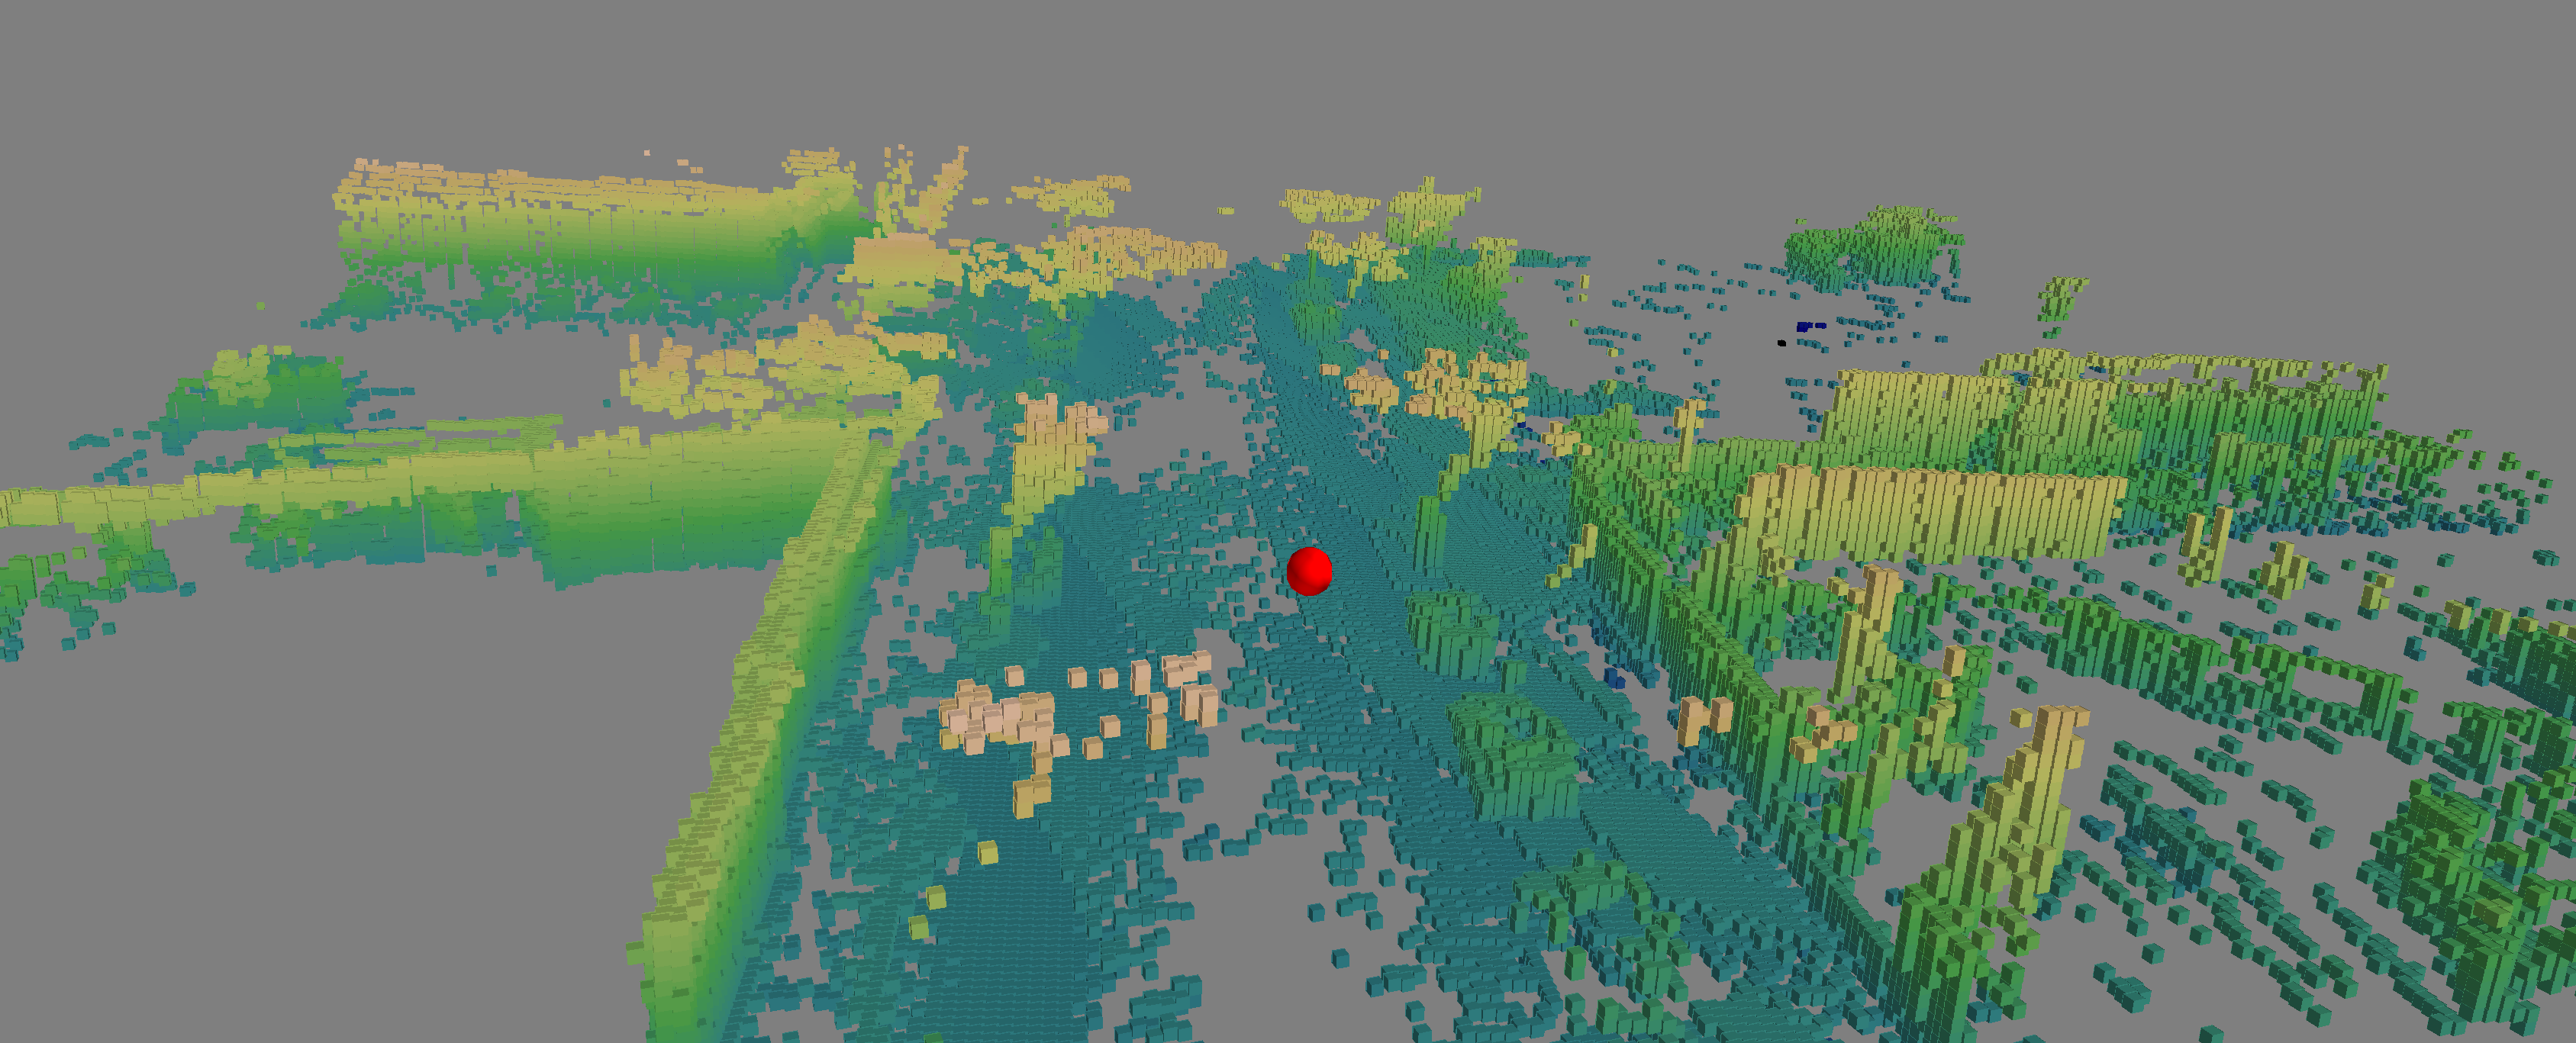
\includegraphics[width=0.8\linewidth]{fig/gt.png}

\vspace{1mm}

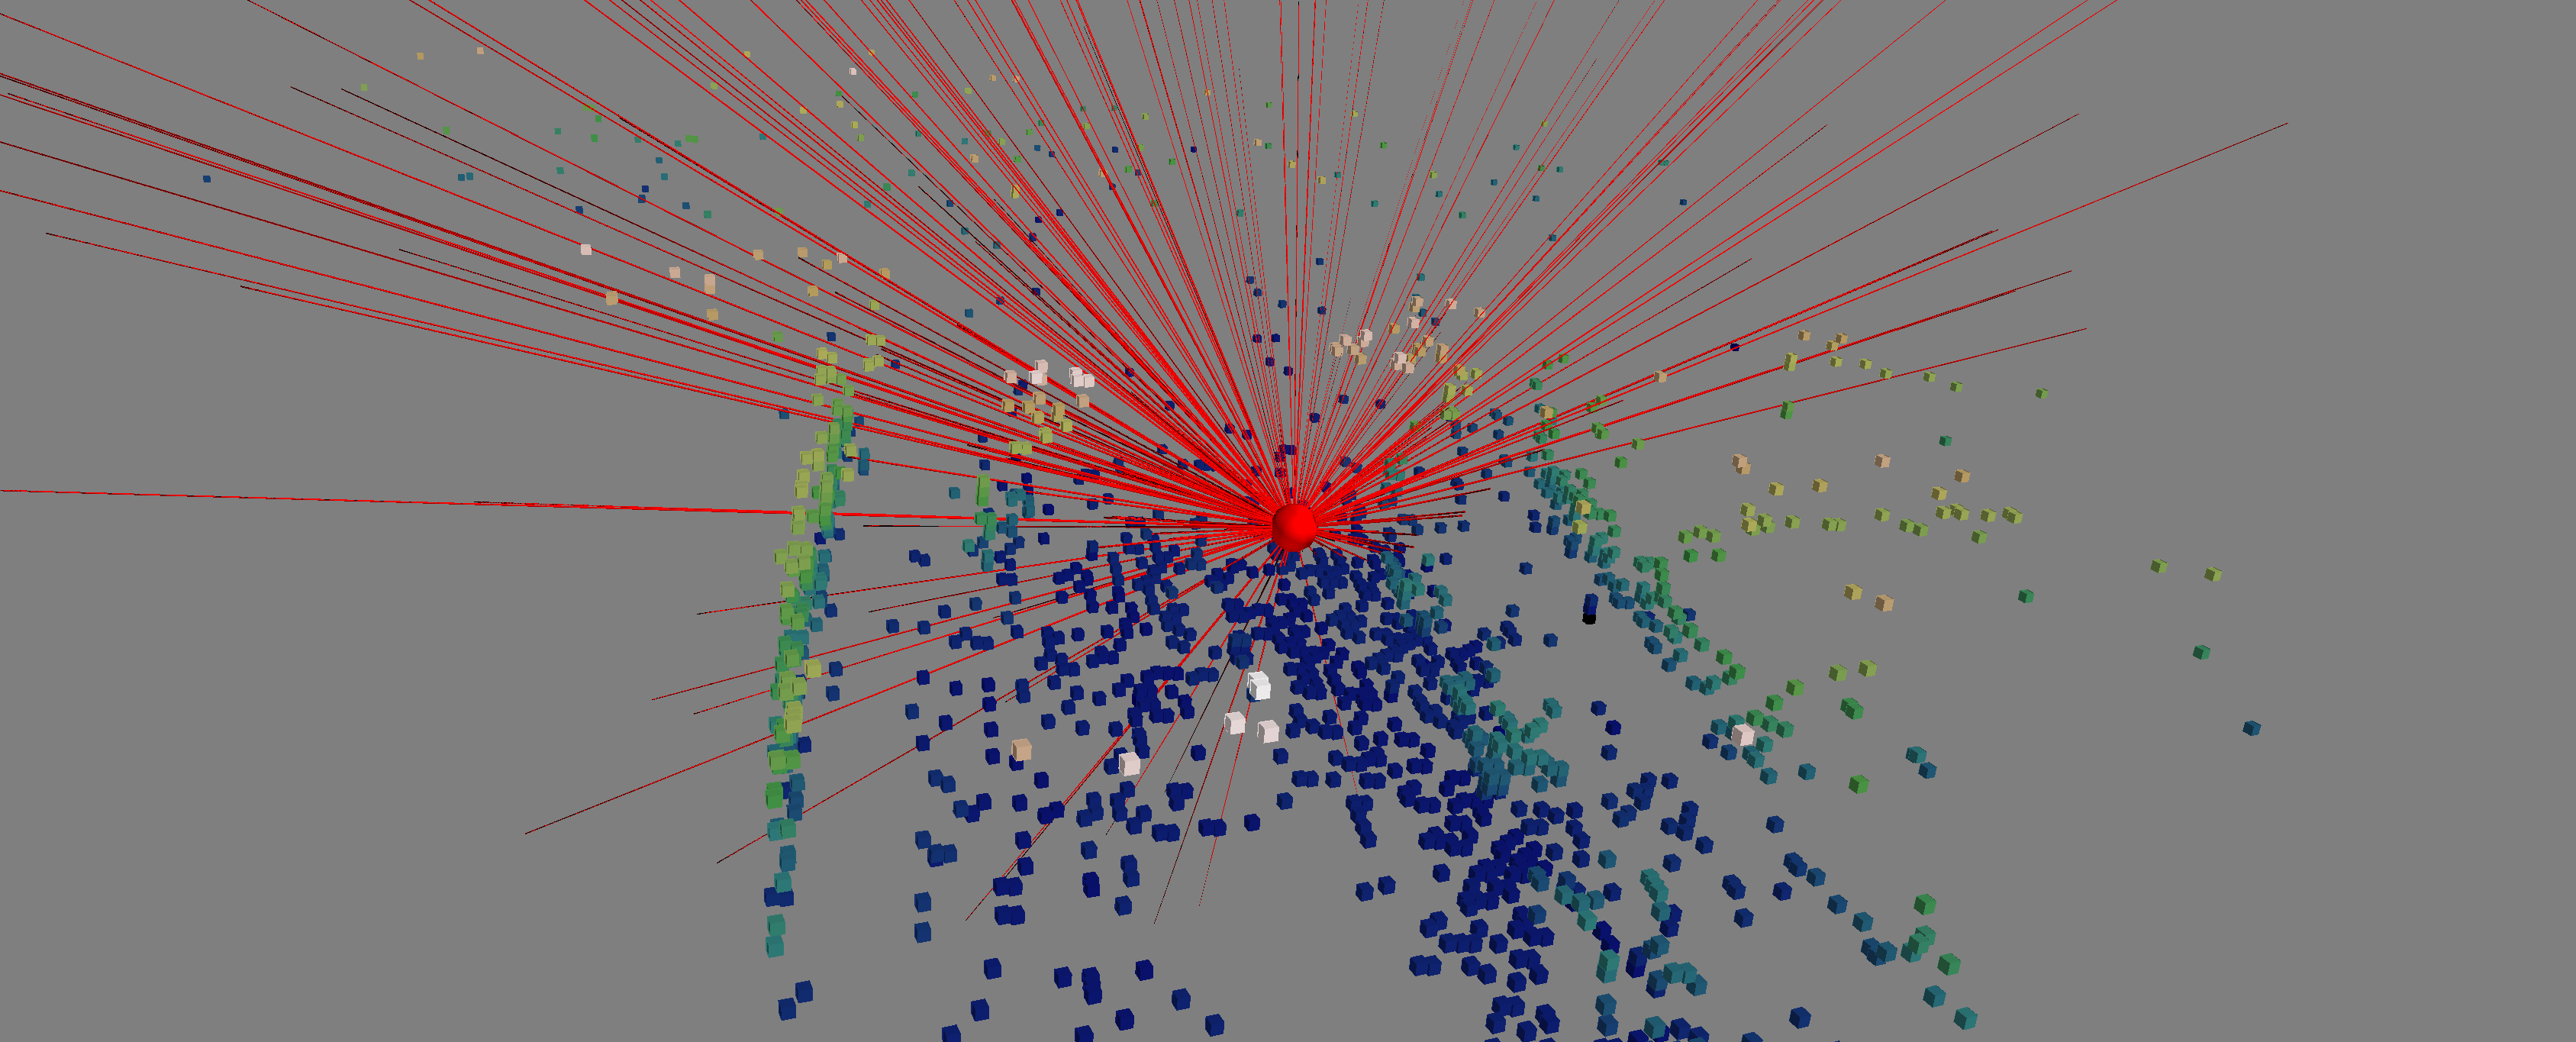
\includegraphics[width=0.8\linewidth]{fig/sparse.png}

\vspace{1mm}

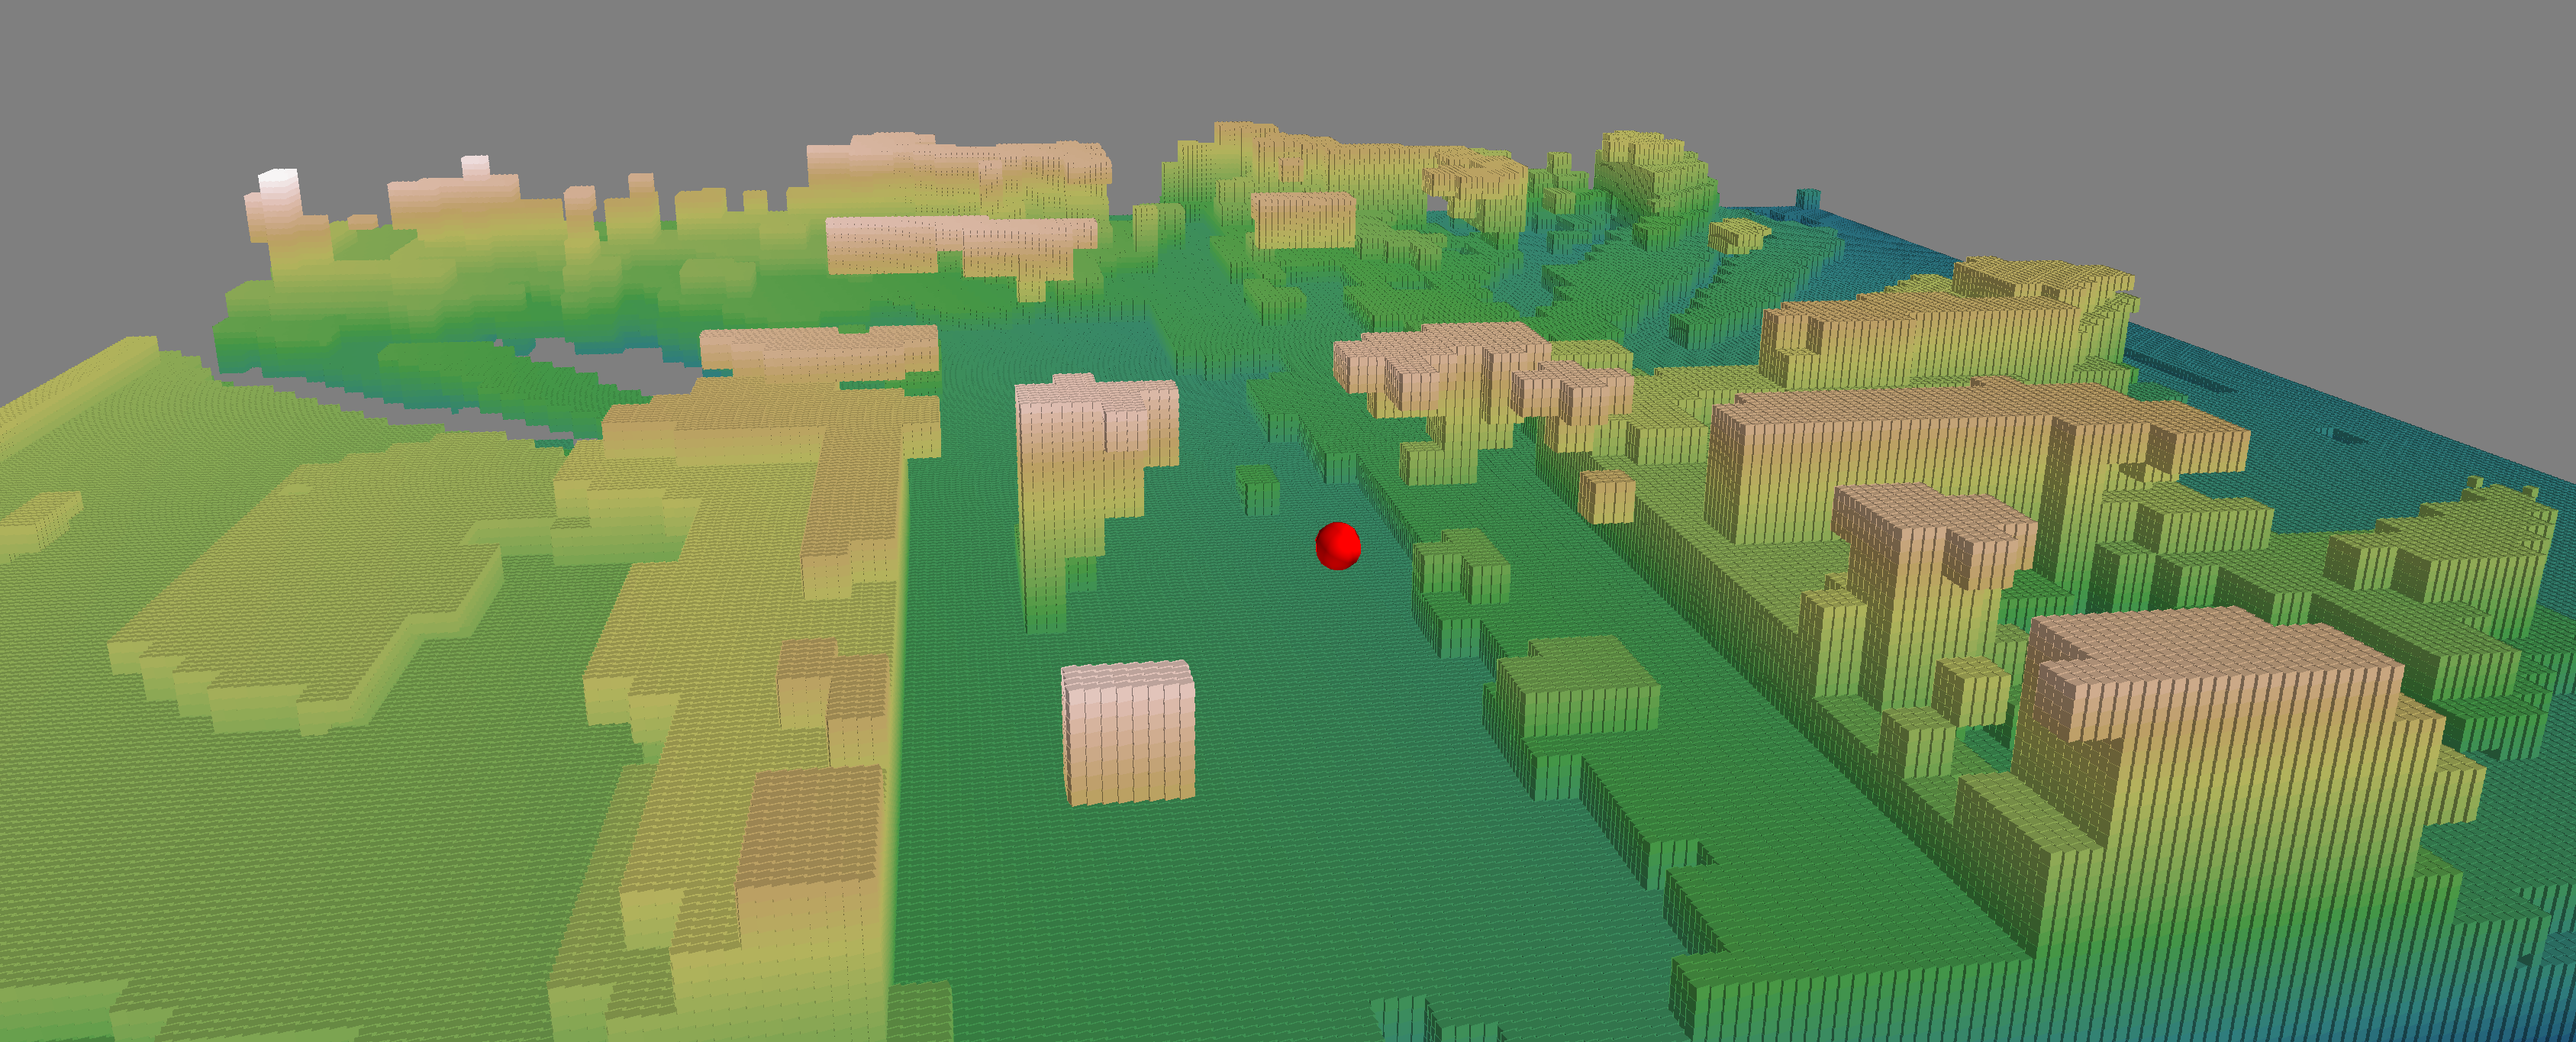
\includegraphics[width=0.8\linewidth]{fig/reconstructed.png}

\caption[Environment visualization]{Visualization of the large environment: The first figure is the ground truth map, second is the voxel map of the sparse measurements and the third figure shows the dense reconstruction. The dense reconstruction in the third figure and the rays fired in the second figure are made by an agent using the random planner. Some known structures as cars and trees can be seen in the reconstructed map.}
\label{fig:visualization}
\end{figure}

\clearpage
Due to the high time complexity, all experiments were conducted in the toy environment. The RL agents need significantly more training steps than supervised agents. Unlike the RL agents, for the supervised agent is known desired output, thus it can be learned by a gradient descent on the loss function between made and desired outputs. There are the RL agents trained for over million epochs in OpenAI baselines \cite{openai2017}. A drive in the KITTI dataset has on average 200 epochs. All agents were trained and evaluated on different drives from the city category of the dataset.

\subsection{Mapping agent}
The mapping agent is based on work of Zimmermann et al. \cite{zimmermann2017}. It uses a convolutional neural network (CNN) for reconstructing the dense map from the sparse measurements. 3D convolutional layers are used to learn features and max-pooling layers are used to avoid overfitting. The CNN architecture is described in Figure \ref{fig:supervised}.
\vspace{3mm}
\begin{figure}[!h]
\centering
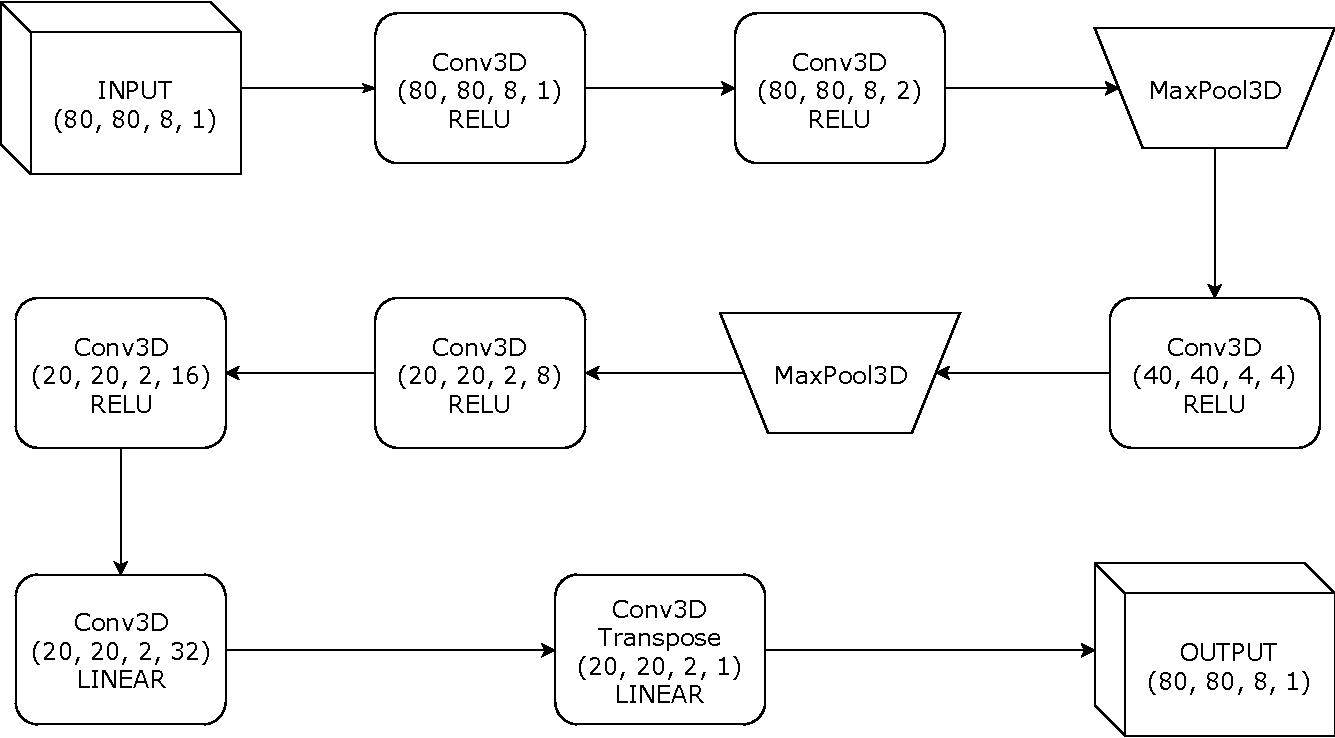
\includegraphics[scale=0.6]{fig/supervised.pdf}
\caption[Mapping network architecture]{Input of the supervised mapping agent is voxel map containing the sparse measurements. The output is the dense reconstruction of the input.}
\label{fig:supervised}
\end{figure}

Gradient descent is made by Adam optimizer \cite{adam2014}. Optimizer uses a logistic loss $L$ between a ground truth map $Y$ and predicted dense map $\hat{Y}$.
\begin{equation} \label{eq:loglos}
L(Y, \hat{Y}) = \sum\limits_i w_i \log(1 + \exp(-Y_i \hat{Y_i}))
\end{equation}
where $w$ are weights which balance importance of the occupied and unoccupied voxels.
\pagebreak
Unfortunately, a naive implementation of this loss function is computationally inconvenient and often cause numerical issues as overflow. To stabilize training, the following modified loss was used \cite{matconvnet2015}
\begin{align} 
\begin{split}
a_i &= -Y_i \hat{Y_i} \\
b_i &= \max(0, a_i) \\
L &= \sum\limits_i w_i (b_i + \log(\exp(-b_i) + \exp(a_i-b_i))).
\end{split}
\end{align}
At first, the supervised mapping agent with a random ray planning is trained. Reconstructions of the supervised agent are then used for the training of the RL planning agents and after that is the mapping agent retrained with the RL agent picking the rays.
\subsection{Discrete planning agent}
Since the action of the environment $A_t$ for directions of the rays is 2D binary array, first try is to use a discrete agent. The DQN is the most used option for discrete action space, but in this use case, it requires some tweaks. Note that the number of the possible actions is extremely large. Even in the toy environment it is $40\times30 \choose 15$ $\approx 10^{34}$ of actions. Thus it is necessary to emphasize the action space exploration. Further arises the problem with the $\epsilon$-greedy policy, because we are unable to process all the possible actions and pick the one with the biggest Q-value. We consider only one ray as action to resolve this issue. For $K$ rays is the TD from \eqref{eq:qlearn} now computed as:
\begin{align} \label{eq:dql}
\begin{split}
q(S_t, A_t) &= \max\limits_{A_t}^K Q^\theta(S_t, A_t)\\
\delta_t &= R_t + \gamma \overline{q}(S_{t+1}, A_{t+1}) - \overline{q}(S_t, A_t)
\end{split}
\end{align}
where $\overline{q}$ is an average $Q$ value over $K$ actions with maximum $Q$ values. The DQN agent implements all features as Prioritized experience replay, target network, and double Q learning which are described in the theoretical part of this thesis. The exploration is ensured by the action space noise. The neural network architecture is described in Figure \ref{fig:dqn}. The agent uses values of parameters shown in Table \ref{tab:params}. The weights are updated via stochastic optimizer Adam with learning rate $\lambda$.

\clearpage
\begin{figure}[!h]
\centering
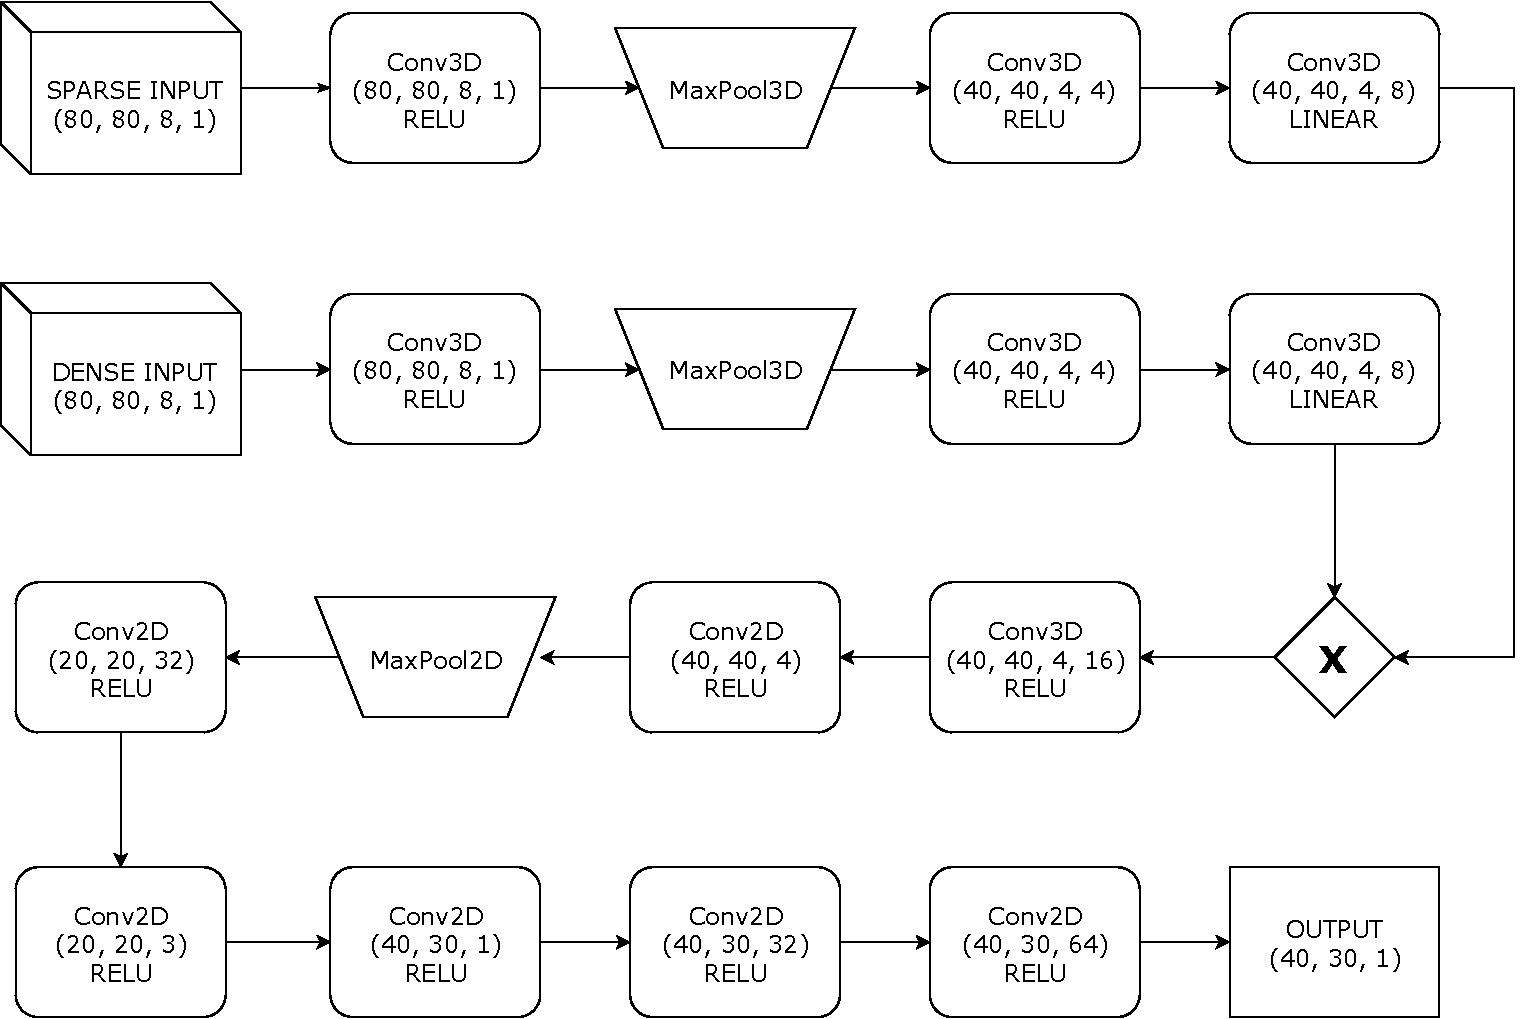
\includegraphics[scale=0.6]{fig/dql.pdf}
\caption[DQN architecture]{The DQN outputs an estimate of the Q-value. The network takes as the input two voxel maps. In conducted experimets was significantly better to merge these two inputs using multiplication than using addition.}
\label{fig:dqn}
\end{figure}

\clearpage
\subsection{Continuous planning agent}
The discrete action output was substituted by a continuous action, which is then mapped into the 2D binary array. This will allow the agent to avoid the extremely large discrete action space. Thank to this substitution it is possible to exploit the actor-critic framework. The output of the actor is now $2$ by $K$ array where the first row is the elevation and the second row is the azimuth of each ray. The last layer of the actor-network is tanh function, so its output is an element of $[-1, 1]$. As training method is used DDPG. The neural network architecture is described in Figure \ref{fig:ddpg}.

\begin{figure}[!h]
\centering
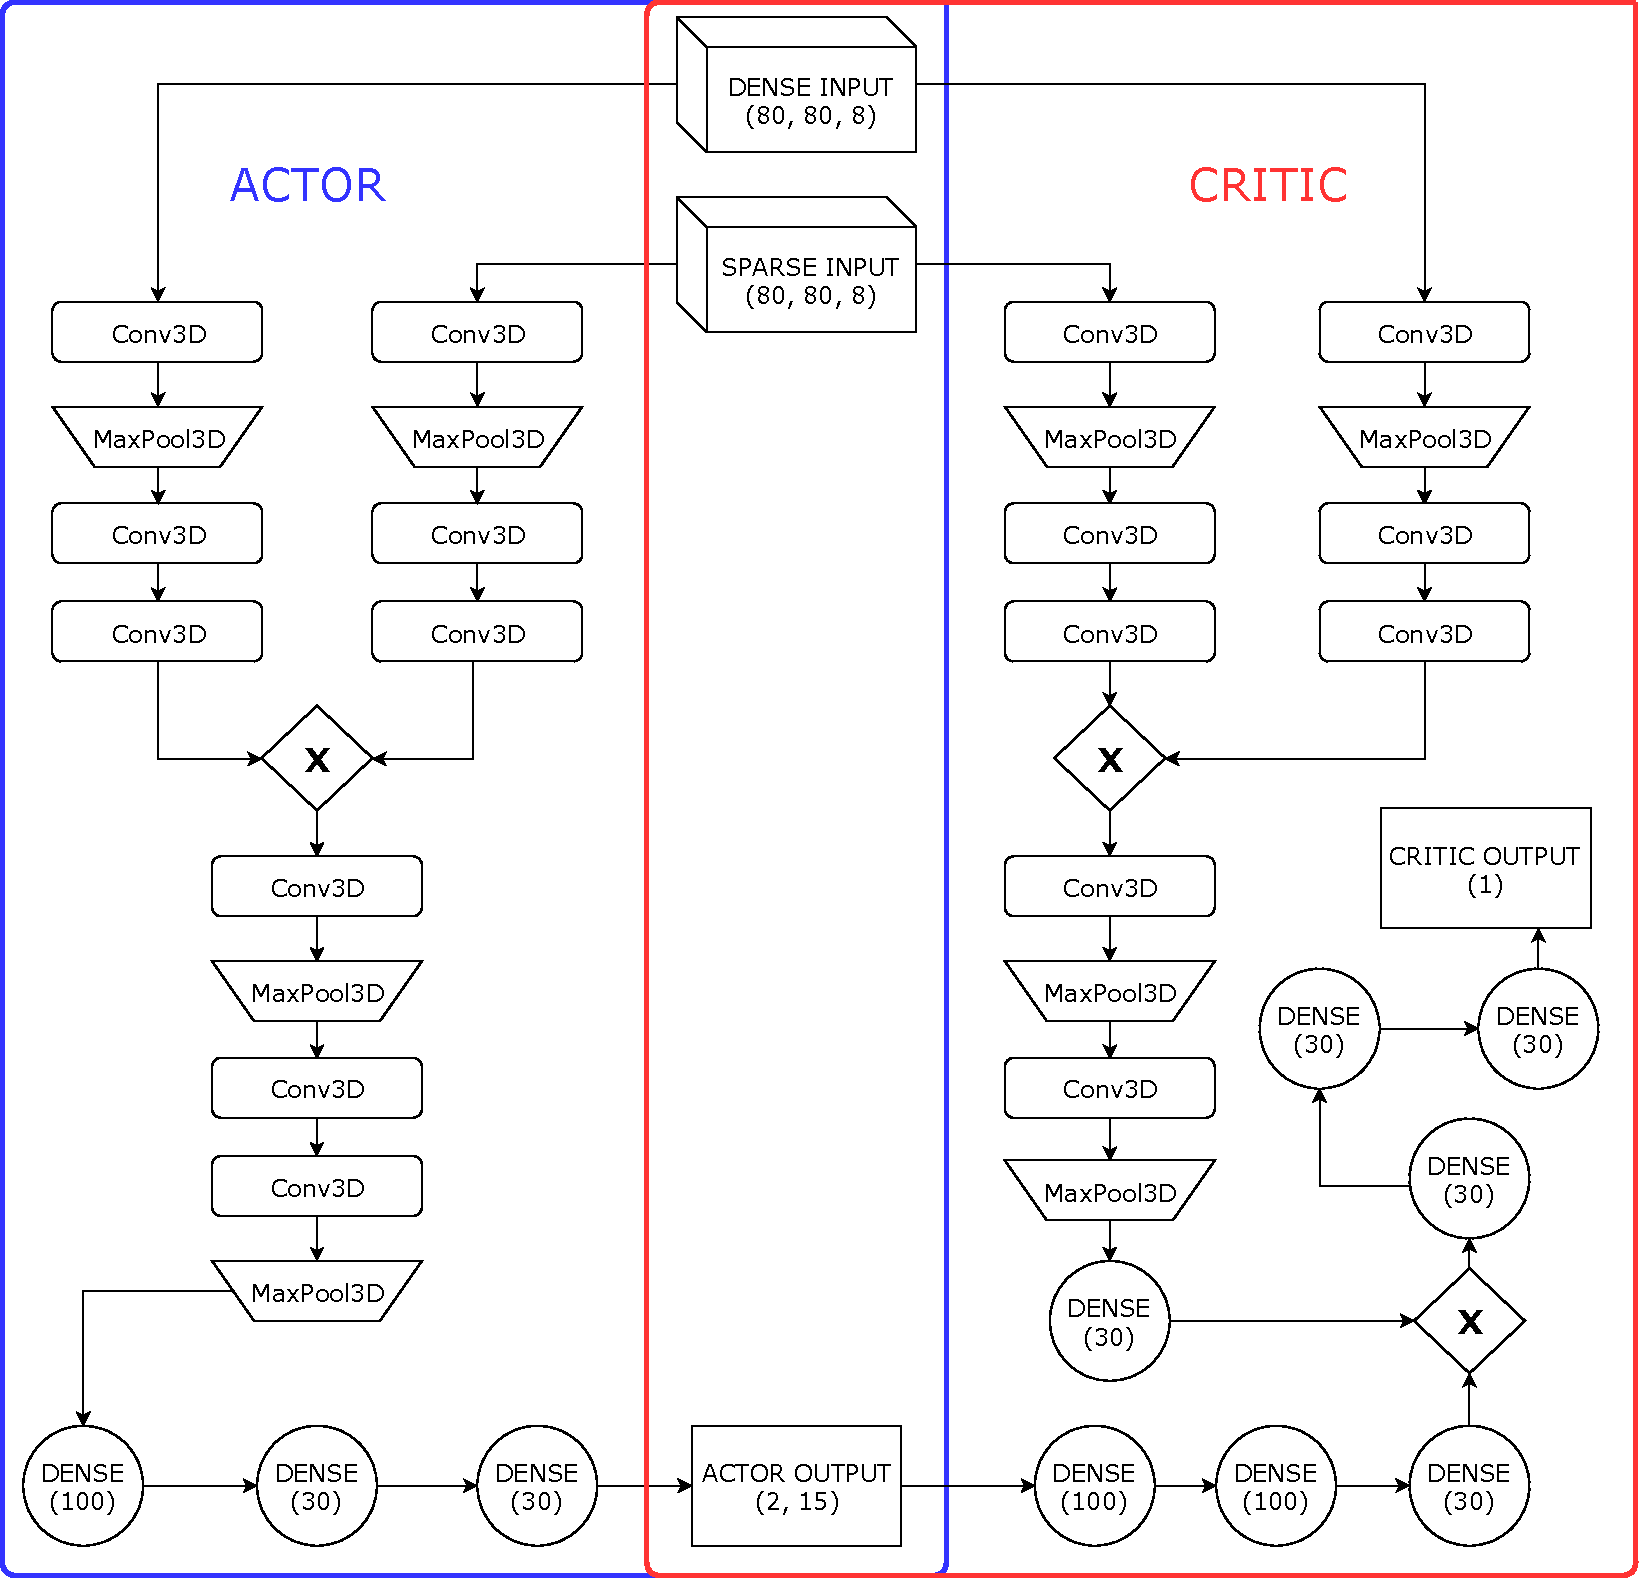
\includegraphics[scale=0.55]{fig/ddpg.pdf}
\caption[DDPG architecture]{The architecture of the actor is on the left side and the critic is on the right side. In the middle can be seen shared inputs and outputs.}
\label{fig:ddpg}
\end{figure}

\pagebreak
To explore the action space in our experiments correctly, it is necessary to apply Ornstein-Uhlenbeck random process. When only Gaussian noise is added, actions tend to converge into the corners very fast as in Figure \ref{fig:expdiff}. For actor's and critic's neural network is used Adam optimizer with learning rates $\lambda_{a}$, $\lambda_{c}$. The target networks are used to stabilize the learning of the actor and critic. The continuous agent also uses prioritized experience replay.

\begin{figure}[H]
\begin{subfigure}[h]{0.5\linewidth}
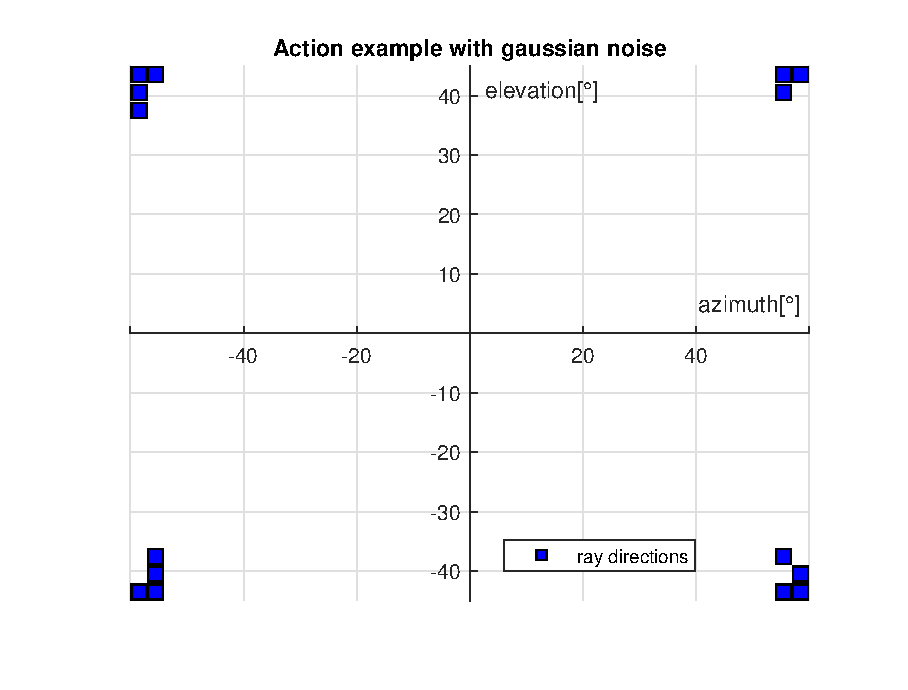
\includegraphics[width=\linewidth]{fig/wrong_action.eps}
\end{subfigure}
\hfill
\begin{subfigure}[h]{0.5\linewidth}
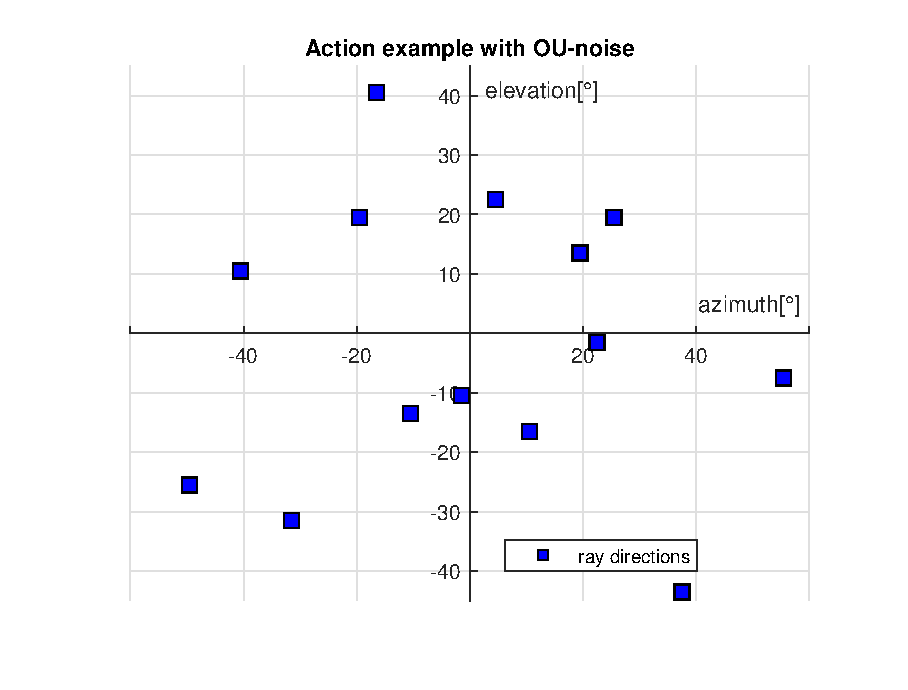
\includegraphics[width=\linewidth]{fig/right_action.eps}
\end{subfigure}
\captionsetup{width=1\textwidth}
\caption[Difference between exploration methods]{The difference between actions made by agents with the different exploration methods. Left figure is an example of the action made by an agent with Gaussian noise used for the exploration. The action in the right figure is made by the agent trained using Ornstein-Uhlenbeck noise.}
\label{fig:expdiff}
\end{figure}

\subsection{Stochastic planning agent}
There is an obvious issue with the deterministic actor. For efficient exploring of the ground truth map, it is required to hit as many unique voxels as possible. Thus making several similar actions in a row is not a good strategy. Unfortunately, except the first few epochs of every drive, there is not a big difference between two subsequent observations. It is hard for a neural network to make two different outputs for two similar inputs. The solution to this problem could be a stochastic agent. The stochastic agent outputs parameters of the Beta distribution and preserves the Actor-Critic framework. The architecture of stochastic agent is similar to the DDPG from the previous subsection, the only difference is that the agent now outputs only two values - the distribution parameters. The action is then sampled with distribution probabilities. Stochastic actor output can be seen in Figure \ref{fig:stochaction}.

\clearpage

\begin{figure}[H]
\centering
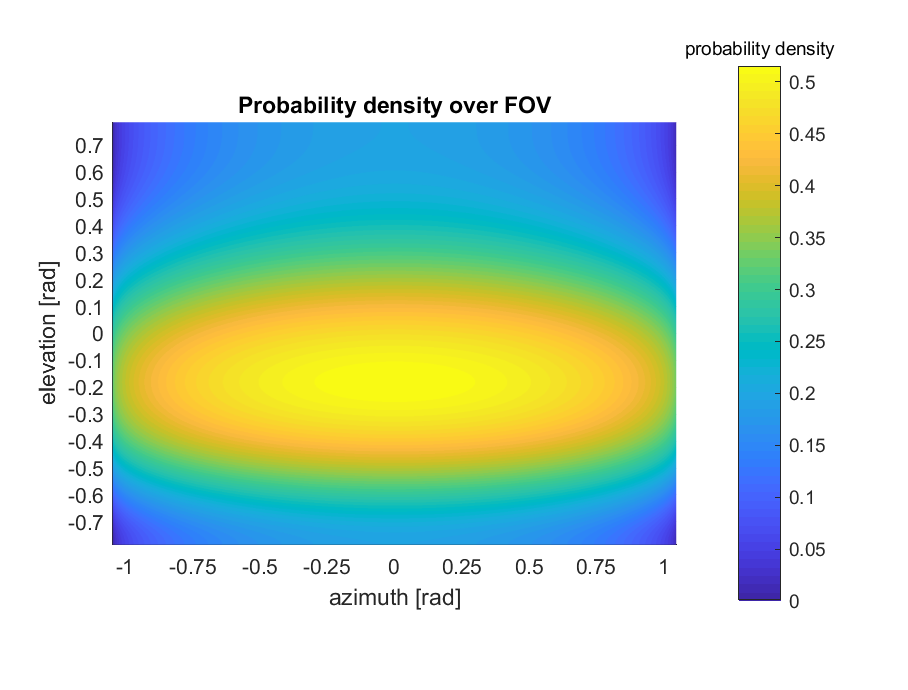
\includegraphics[width=0.85\linewidth]{fig/betapdf.eps}
\caption[Example of stochastic actor output]{The example of stochastic agent output - probability density of choosing a ray with specific azimuth and elevation.}
\label{fig:stochaction}
\end{figure}

\subsection{Comparison of methods}
Several methods were tried. Unfortunately, most of the methods do not perform well in the Lidar-gym environment. The DQL had the worst performance. That is probably caused by the extremly large action space. The workaround made in formula \eqref{eq:dql}, did not help the agent to converge. The continuous DDPG agent also did not converge successfully. For DDPG agent is hard to change direction of the rays efficiently in the subsequent epochs and it often makes several same actions in a row which degrades performance a lot. Only the stochastic agent was able to outperform a random agent. Summary of the agents performances is made in Figure \ref{fig:roc}. It turns out that it is very difficult to get satisfying results. The stochastic agent converges, but it does not use any kind of the advanced strategy. The output of the DDPG actor does not even allow making any sophisticated action. Therefore were also conducted experiments with an extended stochastic agent, which uses the Beta distribution for each ray separately, but with no significant success. Another advantage of the simple stochastic agent is its scalability. This agent can be adjusted to the large environment much easier than any other used agent. The parameters used for the training of these agents are described in Table \ref{tab:params}.

\clearpage

\begin{table}[h!]
  \centering
  \begin{tabular}{*{2}{c}}
    \toprule
    Parameter & Value \\
    \midrule
    $\gamma$ & 0.09 \\
    $\lambda_{c}$ & 0.001 \\
    $\lambda_{a}$ & 0.0001 \\
    $\tau$ & 0.01 \\
    Memory size & 4096 \\
    Batch size & 8 \\
    \bottomrule
  \end{tabular}
  \caption[Learning parameters]{Parameters used for learning. DQN uses $\lambda = \lambda_{c}$.}
  \label{tab:params}
\end{table}

\begin{figure}[h!]
\centering
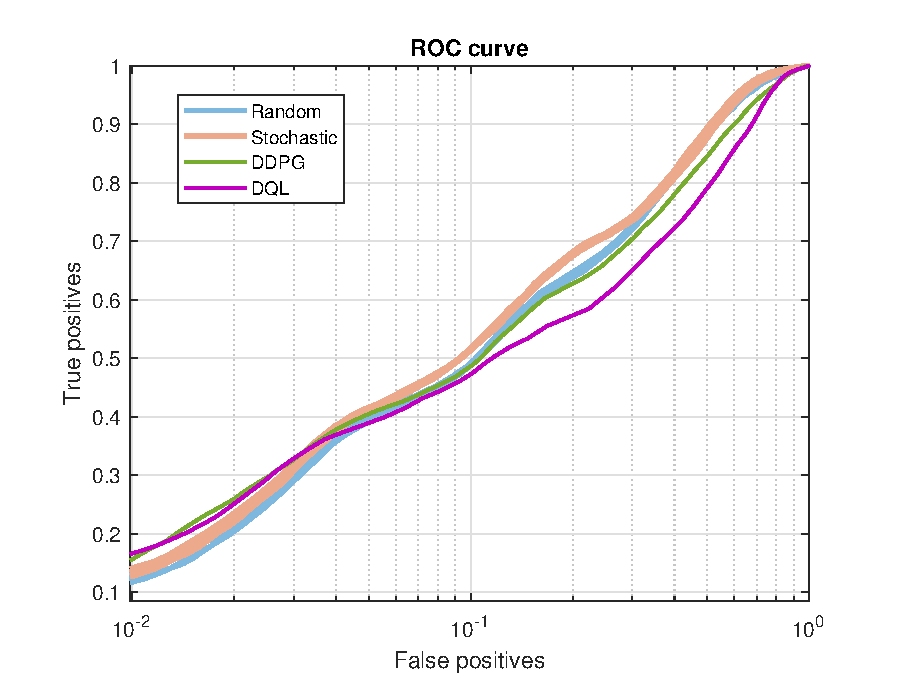
\includegraphics[width=1\linewidth]{fig/roc.eps}
\caption[ROC curves comparison]{False positives were calculated using the ground truth map and true positives using all voxels, which could be possibly hit by the sensor. Five different evaluations are displayed for the non-deterministic agents.}
\label{fig:roc}
\end{figure}

\clearpage


